\documentclass{f4_beamer_metropolis}

\newcommand{\iu}{{i\mkern1mu}}

\newcommand\blfootnote[1]{%
  \begingroup
  \renewcommand\thefootnote{}\footnote{#1}%
  \addtocounter{footnote}{-1}%
  \endgroup
}

\title{Realistic real-time rendering of skin under consideration of physical basis}
\subtitle{Master seminar SS2020}
\author{Dennis Grabowski, B.Sc}
\date{25.05.2020}

\bibliography{paper.bib}

\begin{document}

% Cannot be moved into the class
\begin{frame}[t]{Table of contents}
    \tableofcontents[hideallsubsections]
  \end{frame}

\section{Prologue}
\label{sec:intro}

\begin{frame}[t]{Did we learn everything about light?}
  \begin{itemize}
    \item Until now, we learned light either ...
    \begin{itemize}
      \item ... reflects away from an object or
      \item ... refracts into an object
    \end{itemize}
    \item What happens to the light ray after refracting into the object?
    \item What happens if the object consists of multiple materials?

    \note{
      While refracting was happily explained by Artur Ritter on 18.05.2020, a reminder will be given and further explanation to the light rays in an object/heterogenous medium
    }
  \end{itemize}
\end{frame}

\begin{frame}[t]
  \frametitle{Reminder to refraction}
  \begin{itemize}
    \item The effect of material on light is defined by the refractive index
    \item Refractive index can be expressed as complex number: $$ \underline{n} = n + \iu * K$$
    \item real part describes how material affects speed of light (i.e. slowing it down relative to its speed in a vacuum)
    \item complex part determines whether light is absorbed as it propagates through the medium
  \end{itemize}
\end{frame}

\begin{frame}[t]
  \frametitle{Different mediums, different refractions}
  \begin{itemize}
    \item Transparent medium:
      \begin{itemize}
        \item Always the same refractive index
        \item No significant absorption,
        \item Light propagating through medium keeps going in straight line, unchanged
      \end{itemize}
    \item Homogenous medium:
      \begin{itemize}
        \item Always the same refractive index
        \item Can have significant absorption,
        \item Direction does not change, intensity however will
      \end{itemize}
    \item Heterogenous medium:
      \begin{itemize}
        \item Multiple variations in refractive index: different layers, irregularities like air bubbles, foreign/microscopic particles, density variations, ...
        \item Can have significant absorption,
        \item Direction and intensity will change
      \end{itemize}
  \end{itemize}

  \note{
    note that directional changes described here are considered to be after refraction happened \\
    transparent: complex part for visible light wavelengths is very low (glass, water, crystals)\\
    homogenous: tea, beer, coffee, milk, oil, wine\\
    heterogenous: wood, stone, snow, earth, opaque plastic\\
  }
\end{frame}

\begin{frame}[standout]
  Enough reminders - give us the answer to the questions before!
\end{frame}


\begin{frame}[t]
  \frametitle{Ok, sorry!}
  \begin{itemize}
    \item What happens to the light ray after refracting into the object?
    \begin{itemize}
      \item Depends on the material ...
      \begin{itemize}
        \item metals fully absorb the refracted light,
        \item non-metal (dielectrics/insulators) behave as regular, participating media
      \end{itemize}
      \item ... and how fast the refractive index changes
      \begin{itemize}
        \item slow and continuously change \textbf{bends} the light in a curve
        \item abrupt change \textbf{scatters} the light
      \end{itemize}
    \end{itemize}
    \item What happens if the object consists of multiple materials?
      \begin{itemize}
        \item Each layer introduces (abrupt) changes in refractive index
        \item Each layer absorbs, reflects, refracts and scatters light
      \end{itemize}
  \end{itemize}

  \note{
    Metals have very high absorption coefficients (i.e. the complex part of the refractive index) (atleast in visible spectrum) \\
    Regular, participating media exhibits the range of absorption and scattering behaviours as known
  }
\end{frame}

\section{Subsurface scattering}
\label{sec:subsurface}

\begin{frame}[t]{What is subsurface scattering?}
  \begin{figure}[!h]
    \centering
    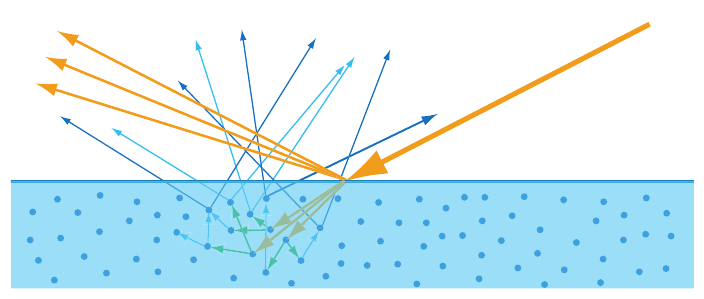
\includegraphics[scale=0.4,keepaspectratio]{./images/subsurface-scattering-illustration.jpg}
    \caption{Illustration of subsurface scattering in dielectric materials}
    \blfootnote{Source: \cite{real-time-rendering}}
  \end{figure}

  \note{
    \begin{itemize}
      \item Light that scatters inside an object consisting of a dielectric material
      \item Scattering does not change overall amount of light
      \item Scattering distribution depends on material and non-uniform
      \begin{itemize}
        \item Unfortunate property for rendering
      \end{itemize}
      \item Some refracted light is scattering such that it is re-emitted out of the same surface, but point of exit is not the same as point of entry
      \item Some refracted light is never re-emitted due to being absorbed while scattering inside the material layer
      \item Absorption inside a material is spectrally variant, i.e. different RGB values
      \item Scattering sometimes allows for spectrally variance, e.g. the sky is blue because blue light scatters more often as it travels in shorter, smaller waves
    \end{itemize}
  }
\end{frame}

\begin{frame}[t]{What is subsurface scattering?}
  \begin{figure}[!h]
    \centering
    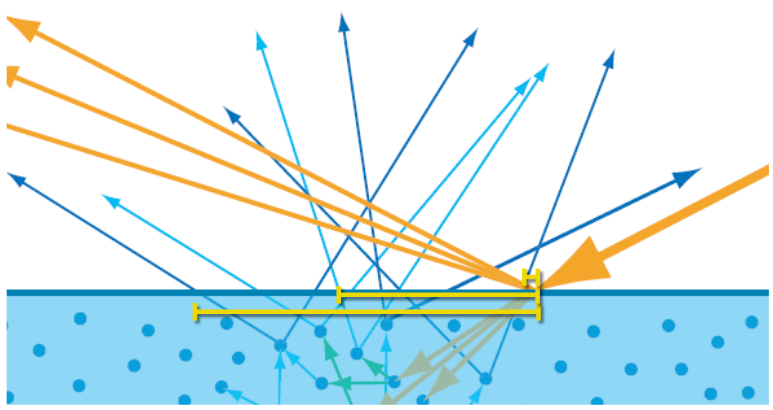
\includegraphics[scale=0.3,keepaspectratio]{./images/subsurface-scattering-distance-difference.jpg}
    \caption{A difference in points of exits compared to point of entry can be seen}
    \blfootnote{Source: \cite{real-time-rendering}}
  \end{figure}

  \note{

  }
\end{frame}

\begin{frame}[t]{What is subsurface scattering?}
  \begin{figure}[!h]
    \centering
    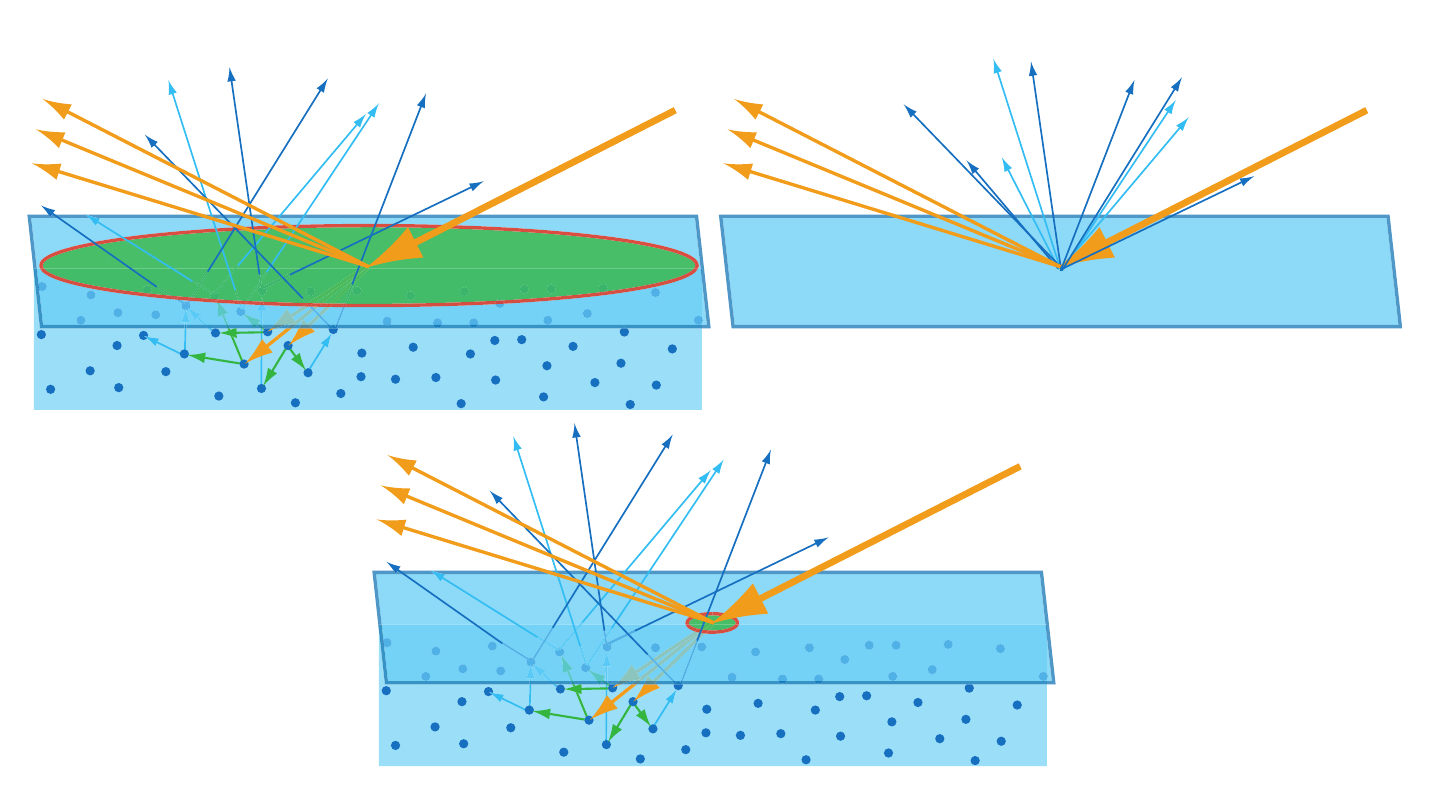
\includegraphics[scale=0.2,keepaspectratio]{./images/subsurface-scattering-pixel-considerations.jpg}
    \blfootnote{Source: \cite{real-time-rendering}}
  \end{figure}

  \note{
    Upper left shows pixel (green circle) is larger than distances traveled by refracted re-emitted light - outgoing light can then assumed to be emitted from entrance point (see upper right). \\
    This assumption is needed for a BRDF, also called local subsurface scattering. \\
    This interesting fact btw allows us to use diffuse shading techniques for skin of a distant character. \\
    Bottom shows scattering distances larger than pixel size, which means that shading of each pixel is depending on all pixels in its neighborhood.\\
    For this, we need a global illumination method. \\
    For realistic rendering, the bottom case cannot be ignored. Which is why rendering some materials realistically is hard.
  }
\end{frame}

\begin{frame}[t]
  \frametitle{Local vs global subsurface scattering}
  \begin{itemize}
    \item Local subsurface scattering can be computed by any BRDF capable of expressing diffuse terms
    \begin{itemize}
      \item Each pixel can be calculated individually
      \item Remember: we consider point of exit == point of entry
    \end{itemize}
    \item Global subsurface scattering is done through methods like \citet{spectral-bssrdf-human-skin}, ray tracing or path tracing.
    \begin{itemize}
      \item Each pixel influences shading of all pixels in their neighborhood
    \end{itemize}
  \end{itemize}
\end{frame}

\begin{frame}[t]
  \frametitle{Single-bounce vs multiple-bounce scattering}
    \begin{itemize}
      \item Single-bounce: Light scatters once inside before re-emitting
      \item Multiple-bounce: Light scatters as often as needed before re-emitting
      \item For most materials: multiple scattering dominates total scattering effect
      \begin{itemize}
        \item ... therefore most research seems to focus on simulating multiple-bounce rendering techniques
      \end{itemize}
    \end{itemize}

\end{frame}

\begin{frame}[standout]
  Ok - can we go back to the skin thing?
\end{frame}

\begin{frame}{Why is this interesting for skin rendering?}
  \begin{figure}[!h]
    \centering
    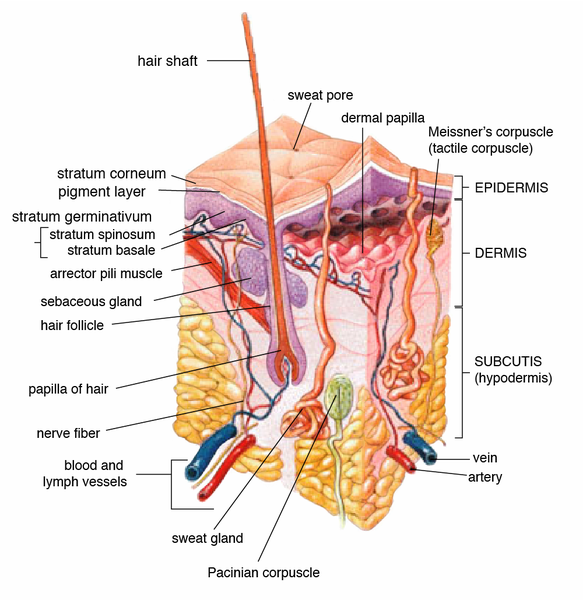
\includegraphics[scale=0.275,keepaspectratio]{./images/skin-layers-medical.png}
    \blfootnote{\scriptsize Credit:\thinspace{\small\itshape \url{https://en.wikipedia.org/wiki/File:Skin.png}}}
  \end{figure}

  \note{
    \begin{itemize}
      \item Skin is a heterogenous medium
      \item Distinct layered structure with hair collicles, wrinkles, sweat glands, capillary veins etcetc
      \item This causes the light to be reflected, absorbed and scattered in multiple, different ways - each interaction different from the layer before.
      \item Stratum corneum is highly scattering, but absorbs almost no light.
      \item Oily substance, sebum, on top of the skin is largely responsible for directly reflected light,
      \item Epidermis, dermis and other layers are responsible for the refracted light. Light scatters amongst these layers and is either absorbed or re-emitted.
      \item The fact below the dermis has very little effect on visible appearance.
      \item According to Tuchin's Tissue Optics paper, roughly 6\% are reflected directly from the skin surface, the rest is scattering in the skin.
    \end{itemize}
  }
\end{frame}

\section{Different subsurface scattering techniques for rendering realistic skin}

\begin{frame}[t]{Different subsurface scattering techniques for rendering realistic skin}
  \begin{itemize}
    \item A BSSRDF - \citep{spectral-bssrdf-human-skin}
    \item \textbf{Texture-Space Diffusion - \citep{efficient-human-skin-rendering}}
    \item Screen-Space Subsurface Scattering (SSSS) - \citep{screen-space-subsurface}
    \item Pre-integrated Subsurface Scattering (PISS) - \citep{pre-integrated-subsurface}
  \end{itemize}

  \note{
    Did not look at all these different methods personally, but to give a quick overview:
    \begin{itemize}
      \item Bold paper is the method we will be looking at
      \item BSSRDF is a generalization of a BRDF that is going to be applied as a global subsurface scattering method
      \item SSSS, also a global subsurface scattering method. Essentially does the same as the selected paper but in Screen-Space - Unity uses this, I think.
      \item PISS - Did not look that hard at this method, The Order: 1886 uses this.
    \end{itemize}
  }
\end{frame}

\subsection{A Spectral BSSRDF for Shading Human Skin}

\begin{frame}[t]
  \frametitle{A Spectral BSSRDF for Shading Human Skin}
  \begin{figure}[!h]
    \centering
    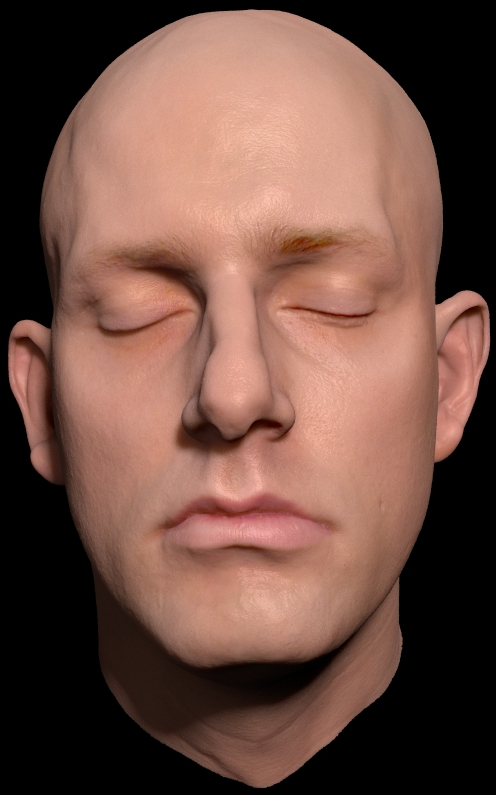
\includegraphics[scale=0.2,keepaspectratio]{./images/bssrdf-head.jpg}
    \blfootnote{Source: \citet{spectral-bssrdf-human-skin}}
  \end{figure}

  \note{
    \begin{itemize}
      \item A global subsurface method scattering that evaluates a BSSRDF per pixel
      \item Uses Torrance-Sparrow (often also called Cook-Torrance) microfacet BRDF for surface reflection
      \item Uses a multipole diffusion model to calculate diffusion profiles that are used for subsurface scattering
    \end{itemize}
  }
\end{frame}

\subsection{Screen-space perceptual rendering of human skin}

\begin{frame}[t]
  \frametitle{Screen-space perceptual rendering of human skin}
  \begin{figure}[!h]
    \centering
    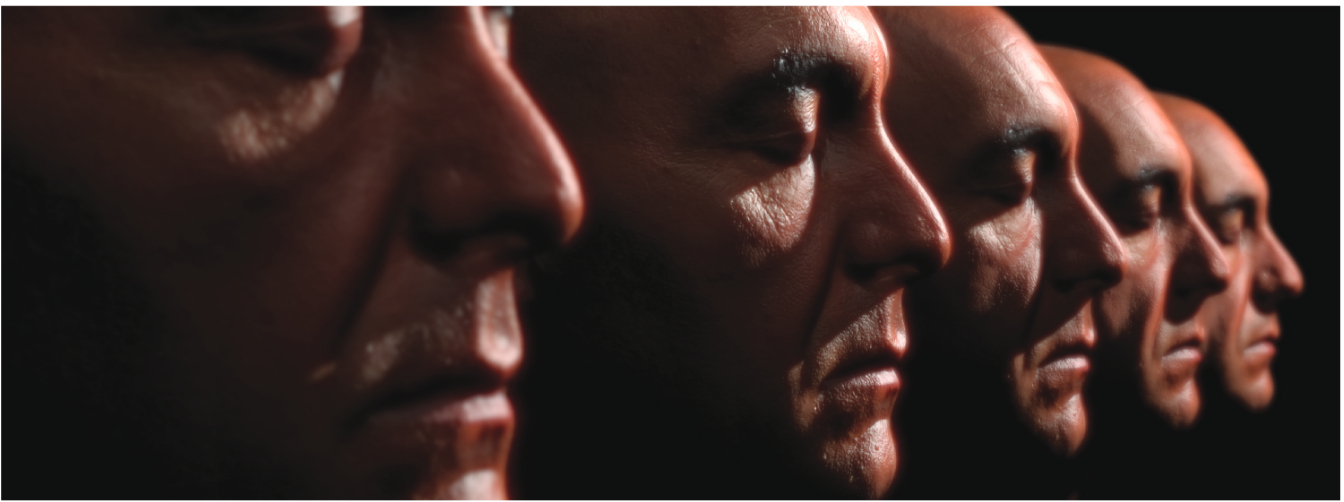
\includegraphics[scale=0.275,keepaspectratio]{./images/screen-space-sss.jpg}
    \blfootnote{Source: \citet{screen-space-subsurface}}
  \end{figure}

  \note{
    \begin{itemize}
      \item Ultimately uses the same technique as the paper we will be looking at, but in screen-space to maximize performance esp. when multiple actors are present.
      \item According to their psychological experiments, other users ranked their results on par with the paper we will be looking at.
    \end{itemize}
  }
\end{frame}

\subsection{Pre-Integrated Deferred Subsurface Scattering}

\begin{frame}[t]
  \frametitle{Pre-Integrated Deferred Subsurface Scattering}
  \begin{figure}[!h]
    \centering
    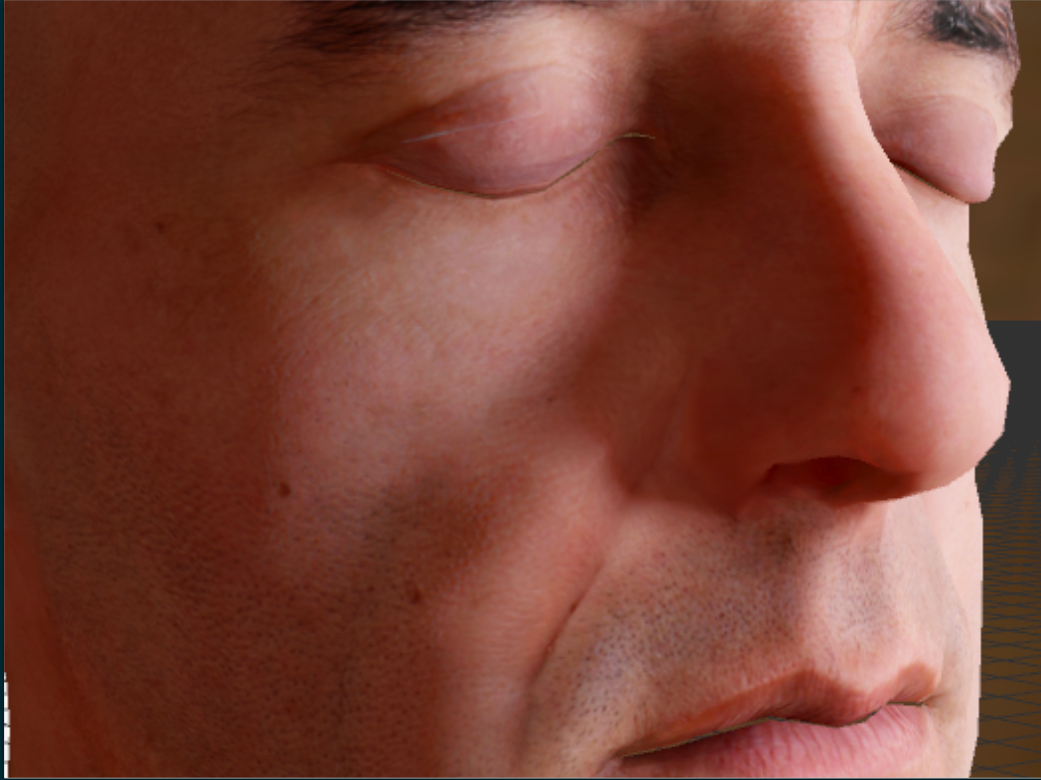
\includegraphics[scale=0.2,keepaspectratio]{./images/pre-integrated-ss.jpg}
    \blfootnote{Source: \citet{pre-integrated-subsurface}}
  \end{figure}

  \note{
    \begin{itemize}
      \item I did not look that hard at this paper, but I wanted to include it to show it's visual results, which frankly, are pretty good
    \end{itemize}
  }
\end{frame}

\section{Texture-Space Diffusion - \citet{efficient-human-skin-rendering}}

\begin{frame}[t]
  \frametitle{About this technique}
  \begin{itemize}
    \item Popularized by \citet{realistic-human-face-rendering-matrix} for the film \enquote{The Matrix}
    \item Formalizes the idea of multiple scattering as a blurring process
    \begin{itemize}
      \item Object mesh unwrapped onto a 2D texture
      \item Computes diffuse lighting on said texture by blurring the light map texture
      \item Reapplies blurred texture back onto the 3D model
    \end{itemize}
  \end{itemize}

  \note{
    \begin{itemize}
      \item Light diffusion is simulated by blurring!
    \end{itemize}
  }
\end{frame}

\subsection{Skin surface reflected light}

\begin{frame}[t]
  \frametitle{Rendering light reflected by skin surface}

  \begin{columns}[onlytextwidth,T]
    \begin{column}{.7\linewidth}
      \begin{itemize}
        \item Kelemen \& Szirmay-Kalos BRDF used: $$f_{diff}(l, v) = albedo * \frac{(1 - R_{spec}(l))* (1 - R_{spec}(v))}{\pi * (1 - \overline{R_{spec}})}$$
        \begin{itemize}
          \item $R_{spec}$ = specular term of the BDRF (sometimes called directional albedo)
          \item $\overline{R_{spec}}$ = cosine-weighted integral over hemisphere
        \end{itemize}
      \end{itemize}
    \end{column}
    \begin{column}{.3\linewidth}
      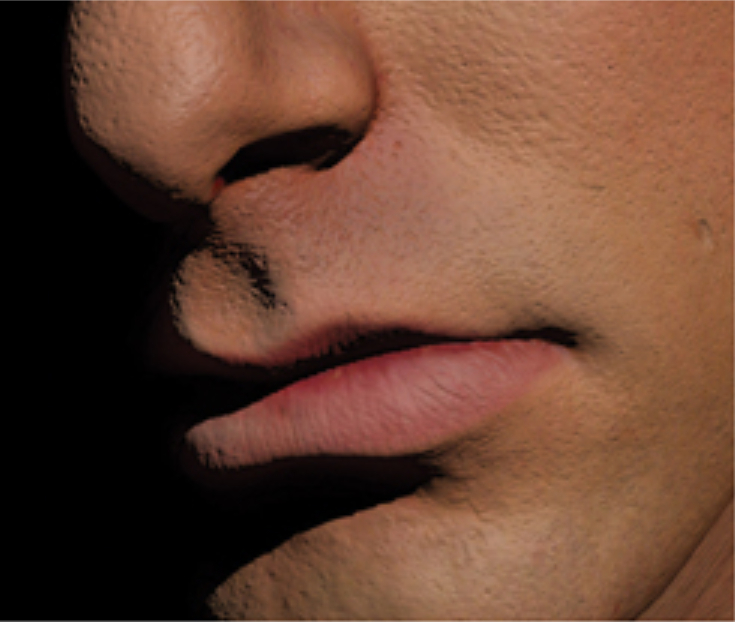
\includegraphics[scale=0.2,keepaspectratio]{./images/skin-rendering-without-sss.jpg}
    \end{column}
  \end{columns}

  \footnote{Formula taken from: \cite[p.~352]{real-time-rendering}, which in turn cites \cite{kelemen2001microfacet}}
  \footnote{Image taken from: \citet{efficient-human-skin-rendering}}

  \note{
    \begin{itemize}
      \item scattering albedo p is ratio between energy of light that escapes a surface compared to energy of light entering into the material
      \item value is between 0 (all light absorbed) & 1 (no light absorbed)
      \item fresh snow or foam on liquid is good example of high scattering albedo - little absorption, immense scattering
      \item good to know/consider is that albedo can have a different spectral distribution and thus color - think of plastic: reflecting specularly light is white, while reflecting diffusely will be colored by the pigment particles of the plastic (i.e. blue)
    \end{itemize}

  }
\end{frame}

\subsection{Skin subsurface reflected light}


\begin{frame}[t]
  \frametitle{Constructing a smaller, multilayer skin model}
  \begin{figure}[!h]
    \centering
    \begin{minipage}{.5\textwidth}
      \centering
      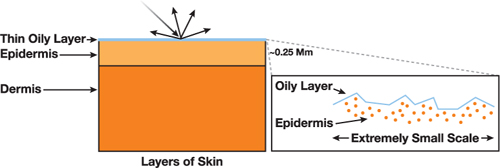
\includegraphics[scale=0.5,keepaspectratio]{./images/multilayer-skin-specular-reflection.jpg}
      \caption{Specular reflection in 3 layer skin model}
      \label{fig:test1}
    \end{minipage}%
    \begin{minipage}{.5\textwidth}
      \centering
      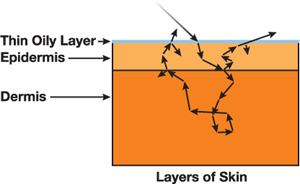
\includegraphics[scale=0.5,keepaspectratio]{./images/multilayer-skin-subsurface.jpg}
      \caption{Subsurface reflection in 3 layer skin model}
      \label{fig:test2}
    \end{minipage}
    \blfootnote{Source: \citet{advanced-realtime-skin-rendering}}
  \end{figure}
\end{frame}

\begin{frame}[t]
  \frametitle{Importance of layer amount}
  \begin{figure}[!h]
    \centering
    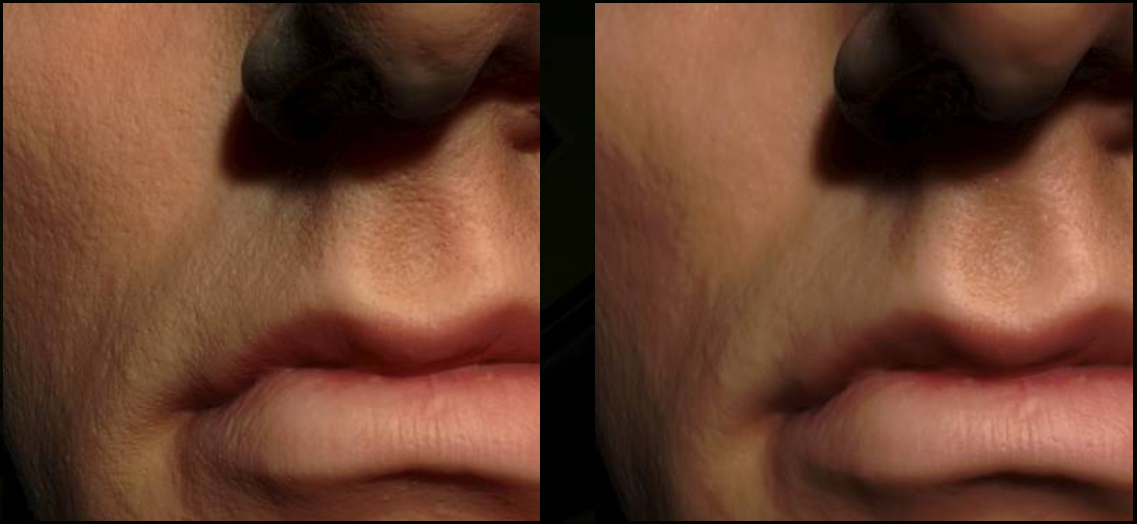
\includegraphics[scale=0.25,keepaspectratio]{./images/importance-of-layer-amount}
      \caption{Left: 3 layer skin model, Right: 1 layer skin model}
    \blfootnote{Source: \citet{efficient-human-skin-rendering}}
  \end{figure}

    \note{
      \begin{itemize}
        \item right side looks waxy
      \end{itemize}
    }
\end{frame}

\begin{frame}[t]
  \frametitle{Diffusion profiles}
    \begin{itemize}
    \item Approximation for light scatter distribution underneath the surface of a highly scattering material
    \item Simple experiment: Illuminating a flat surface in a dark room with a thin, white laser beam.
    \item calculate diffusion profile as sum of gaussians
  \end{itemize}

  \begin{center}
    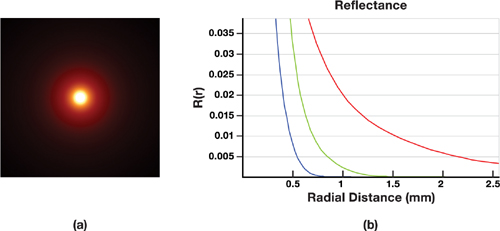
\includegraphics[scale=0.7,keepaspectratio]{./images/diffusion-profile-visualization}
  \end{center}
  \note{
    \begin{itemize}
      \item We are seeing a glowing center which is due to the fact that some light rays are scattering through the surface and returning nearby
      \item This effectively tells us how much light emerges as a function of the angle and distance from laser center
      \item In uniform materials, scattering is the same in all materials, angle irrelevant
      \item Each color has it's own diffusion profile, as some might infer from the right-hand-side.
      \item Donner and Jenson are using 150 different diffusion profiles for their spectral BSSRDF
    \end{itemize}
  }
\end{frame}

\begin{frame}[t]
  \frametitle{A sum-of-gaussians diffusion profile}
  \begin{itemize}
    \item Definition of gaussian distribution: $G(v, r) = \frac{1}{2 * \pi * v} * e^{\frac{-r^{2}}{2*v}}$
    \item $R(r) = \sum\nolimits_{i=1}^k w_i * G(v_i, r)$
  \end{itemize}

  \begin{center}
    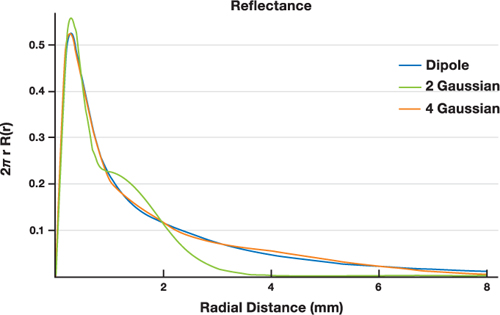
\includegraphics[scale=0.65,keepaspectratio]{./images/approximation-gaussians}
  \end{center}

  \note{
    \begin{itemize}
      \item Authors saw a resembleance in the plotted curves to well-known Gaussian function $e^{-r^2}$
      \item Instead of measuring a diffusion profile for skin, the guys from NVIDIA, approximate the diffusion profile that Donner \& Jensen found in their research
      \item Sums of gaussians seemed to provide excellent Approximation
      \item Gaussians were used because they are simultaneously separable and radially symmetric
      \item $R(r)$ = a diffusion profile
      \item Constant factor in gaussian variance was chosen such that radial 2d blur does not darken or brighten the input image
      \item $r$ stands for radius
      \item find $k$ gaussians with different weights and variances
      \item Authors actually use a six gaussians summation to accurately match the three-layer model given in Donner/Jensen 2005
    \end{itemize}
  }
\end{frame}

\begin{frame}[t]
  \frametitle{Texture-space diffusion}
  \begin{figure}[!h]
    \centering
    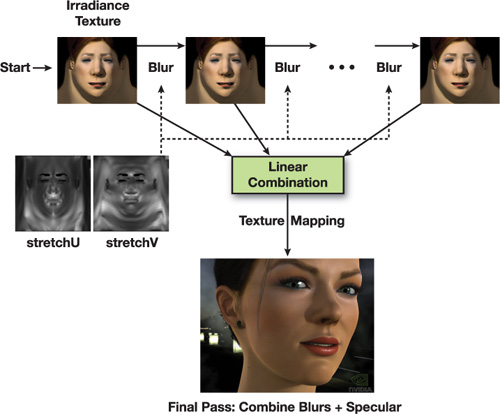
\includegraphics[scale=0.6,keepaspectratio]{./images/texture-space-algorithm.jpg}
    \blfootnote{Source: \citet{efficient-human-skin-rendering}}
  \end{figure}

  \note{
    \begin{itemize}
      \item Rasterize irradiance onto texture via vertex shader (U,V are texture coordinates)
      \item Compute lightning and fresnel terms in fragment shader (excluding specular)
      \item Ultimately more efficient as operations like convolutions can be performed more efficiently in image space
    \end{itemize}

    \begin{enumerate}
      \item Render shadow maps
      \item Render stretch correction map (optional: it may be precomputed).
      \item Render irradiance into off-screen texture.
      \item For each Gaussian kernel used in the diffusion profile approximation:
        \begin{itemize}
          \item Perform a separable blur pass in U (temporary buffer)
          \item Perform a separable blur pass in V (keep all of these for final pass).
        \end{itemize}
      \item Render mesh in 3D:
        \begin{itemize}
          \item Access each Gaussian convolution texture and combine linearly.
          \item Add specular for each light source.
        \end{itemize}
    \end{enumerate}
  }
\end{frame}


\begin{frame}[t]
  \frametitle{Irradiance texture close-up}
  \begin{figure}[!h]
    \centering
    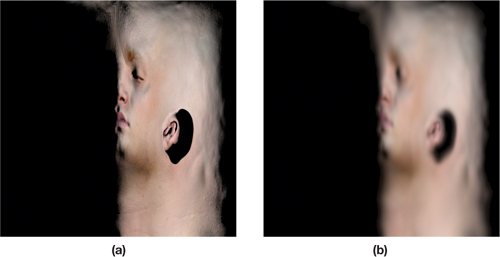
\includegraphics[scale=0.9,keepaspectratio]{./images/irradiance-texture-adrian.jpg}
    \blfootnote{Source: \citet{efficient-human-skin-rendering}}
  \end{figure}
\end{frame}

\begin{frame}[t]
  \frametitle{Texture-space diffusion in visual terms}
  \begin{figure}[!h]
    \centering
    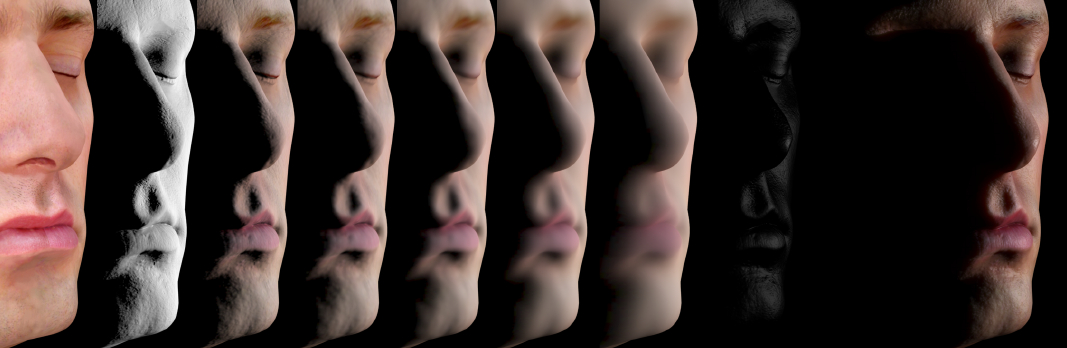
\includegraphics[scale=0.4,keepaspectratio]{./images/human-skin-final-rendering.jpg}
    \blfootnote{Source: \citet{efficient-human-skin-rendering}}
  \end{figure}

  \note{
    \begin{enumerate}
      \item First albedo,
      \item irradiance,
      \item Combine both to calculate subsurface irradiance,
      \item Do all gaussian blurs in texture space
      \item combine with specular
      \item produce final image!
      \item All convulutions are performed in 2d texture space but here mapped onto the face
    \end{enumerate}
  }
\end{frame}

\begin{frame}[t]
  \frametitle{Rendering thin regions such as ears/nostrils correctly}
  \begin{figure}
    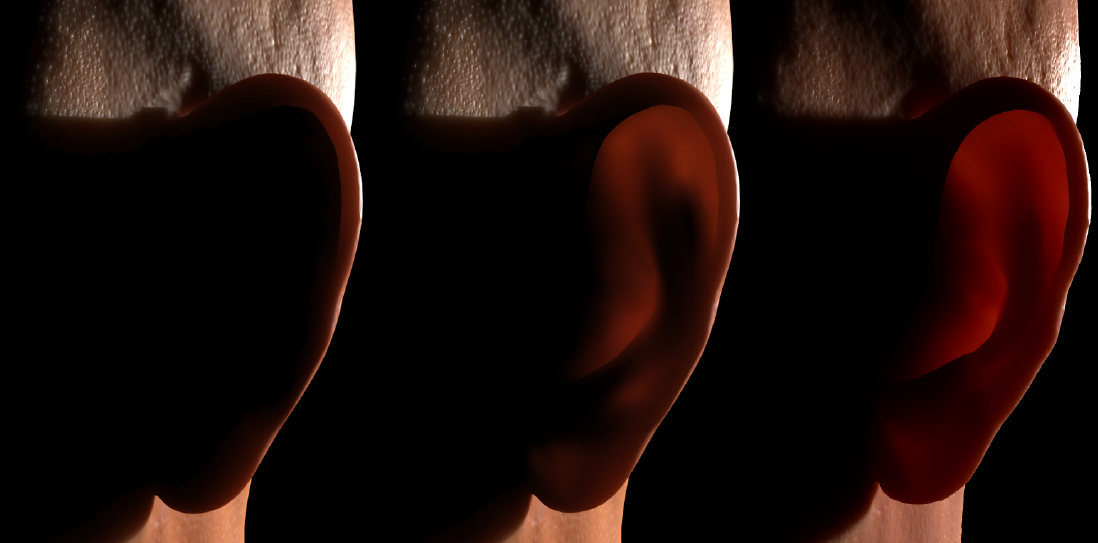
\includegraphics[scale=0.2,keepaspectratio]{./images/translucent-shadow-maps.jpg}
    \caption{
      Left: texture-space diffusion technique in thin skin regions,Center: rendering with translucent shadow maps for thin regions, Right: spectral BSSRDF model from Jensen et al.
    }
    \blfootnote{Image source: \citep{efficient-human-skin-rendering}}
  \end{figure}

  \note{
    \begin{itemize}
      \item Use translucent shadow maps
      \item On ears, nostrils and other thin skin regions the two surface locations are very close in 3D space, but not in texture space which does not correctly calculate the subsurface scattering
      \item \citeauthor{efficient-human-skin-rendering} modified the original maps to allow for a very efficient estimate of diffusion through thin regions by reusing convolved irradiance textures.
      \item Look into my paper for more, think the time is too narrow to go into this.
    \end{itemize}
  }
\end{frame}

\begin{frame}[t]
  \frametitle{Direct comparison of rendering without and with subsurface scattering}
  \begin{figure}[!h]
    \centering
    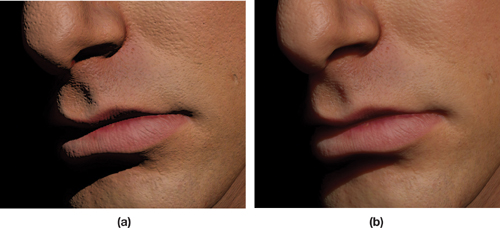
\includegraphics[scale=0.9,keepaspectratio]{./images/skin-rendering-with-without-sss.jpg}
    \blfootnote{Source: \citet{efficient-human-skin-rendering}}
  \end{figure}

\end{frame}

\begin{frame}[t]
  \frametitle{Result with every aspect combined}
  \begin{figure}[!h]
    \centering
    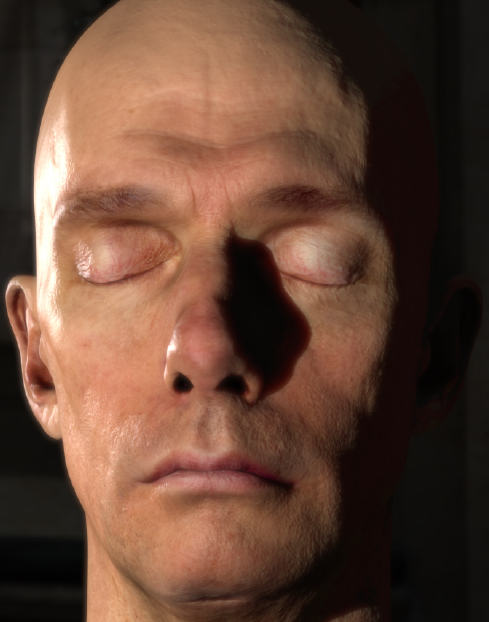
\includegraphics[scale=0.275,keepaspectratio]{./images/nvidia-result.jpg}
    \blfootnote{Source: \citet{efficient-human-skin-rendering}}
  \end{figure}

\end{frame}

\section{Outlook}
\label{sec:outlook}

\begin{frame}[standout]
  Future \textit{real-time} subsurface scattering rendering techniques?
\end{frame}

\begin{frame}[plain]
  \begin{figure}
    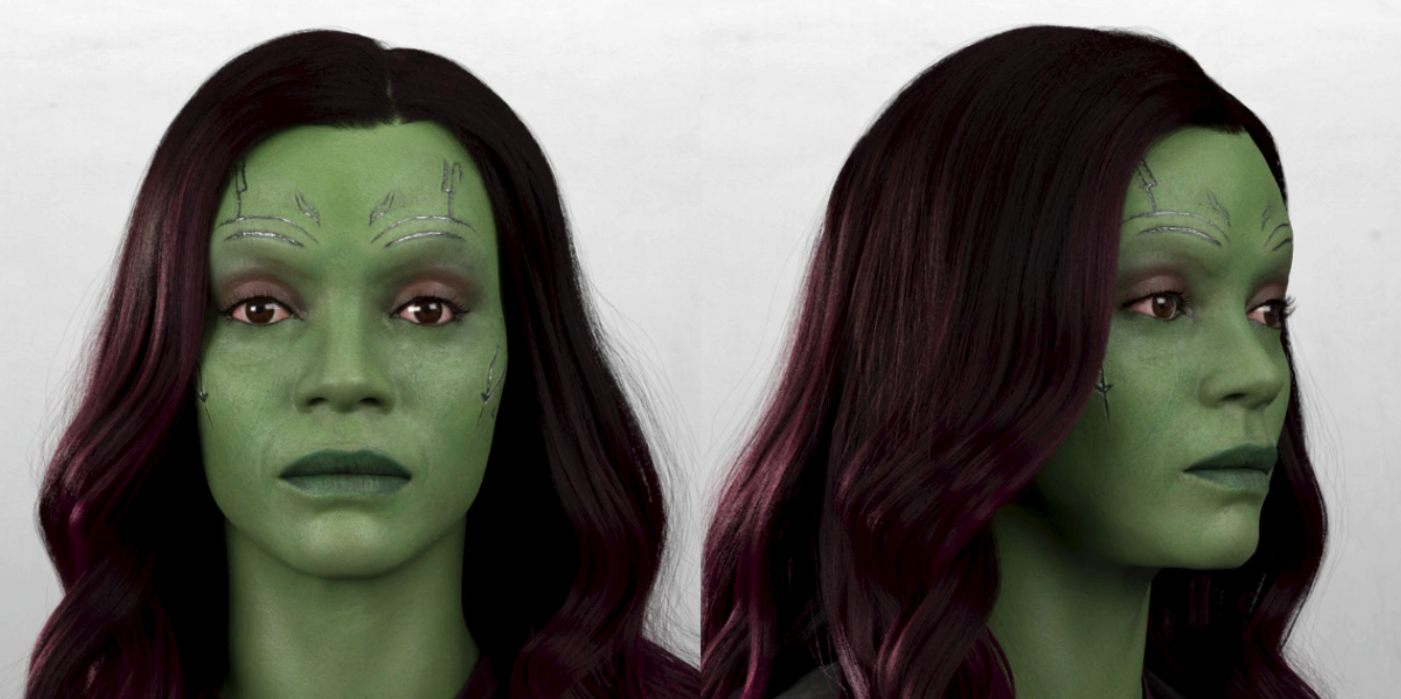
\includegraphics[scale=0.275,keepaspectratio]{./images/framestore-digital-gamora.jpg}
    \caption{Volumetric path tracer - technique used by  Framestore \url{https://blog.selfshadow.com/publications/s2017-shading-course/walster/s2017_pbs_volumetric_notes.pdf}}
  \end{figure}

  \note{
    Framestore is a high-end VFX studio, which did GotG2 and Alien: Covenant effects. \\
    Computationally highly expensive - not usable for anything interactive currently.
  }
\end{frame}

\begin{frame}[plain]
  \begin{figure}
    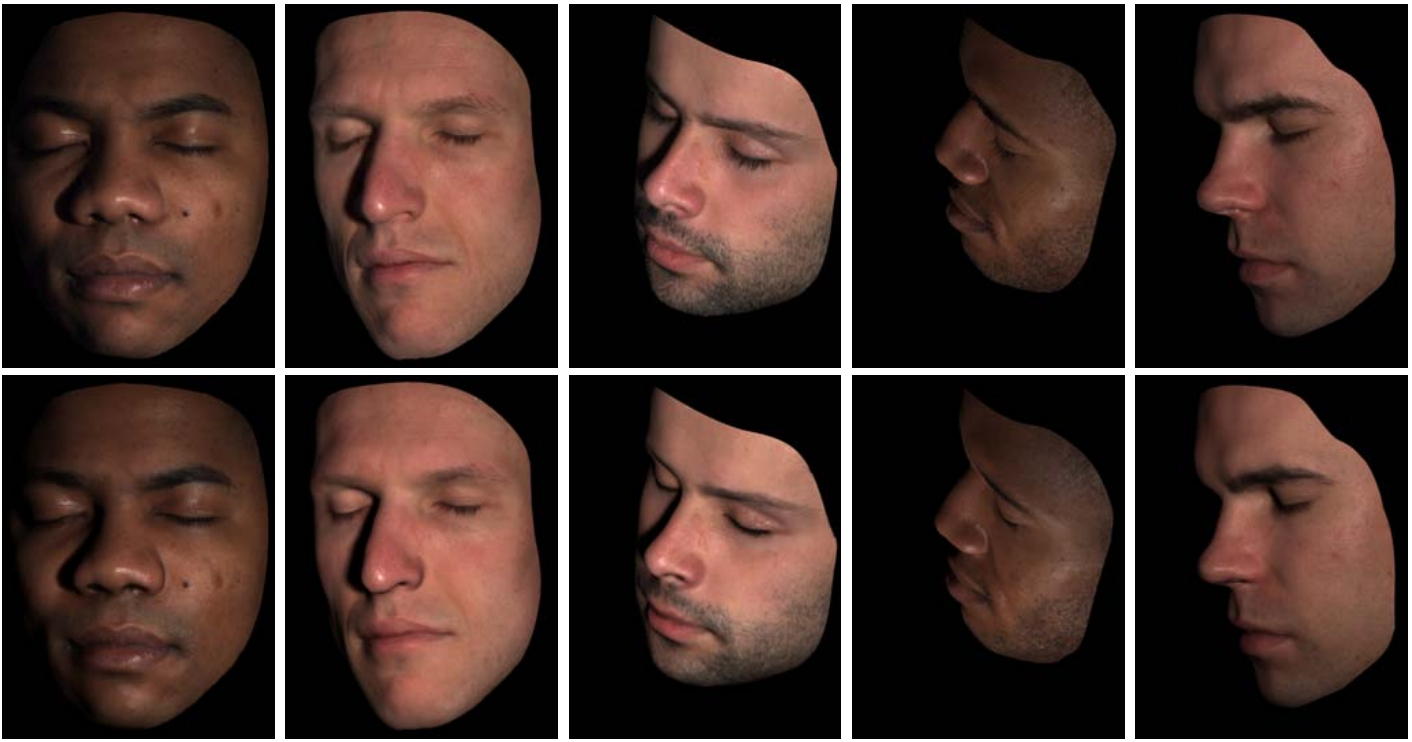
\includegraphics[scale=0.275,keepaspectratio]{./images/monte-carlo-ray-tracer.jpg}
    \caption{A \enquote{Monte Carlo offline ray tracer} implemented in \citet{weyrich2006analysis}. Top row shows photograph, bottom shows rendered images}
  \end{figure}
\end{frame}

\section{Literature}

\begin{frame}[allowframebreaks]{Literature}
  \printbibliography
\end{frame}

\begin{frame}[standout]
  Any questions?
\end{frame}

\end{document}
